% Preprint — Abstract Locks and Transition DAGs. Author: Derek Blair <derekjblair@gmail.com>
% Source data: ~/workspace/math-unsolved/ROUND280_DOSSIER.md (2026-10-10),
%              ~/workspace/math-unsolved/ROUND287_DOSSIER.md (2026-10-11),
%              ~/workspace/math-unsolved/ROUND294_DOSSIER.md (2026-10-10),
%              ~/workspace/math-unsolved/ROUND310_DOSSIER.md (2026-10-11),
%              ~/workspace/math-unsolved/ROUND279_DOSSIER.md (2026-10-10),
%              ~/workspace/math-unsolved/ROUND288_DOSSIER.md (2026-10-11),
%              ~/workspace/math-unsolved/ROUND298_DOSSIER.md (2026-10-10);
%              Lean modules ~/workspace/math-unsolved/lean/Mathproofs/AbstractLock.lean
%              and ~/workspace/math-unsolved/lean/Mathproofs/TransDAG.lean.
% All figures native TikZ/pgfplots; all tables booktabs.
\documentclass[11pt,a4paper]{article}
\usepackage{amsmath,amssymb,amsthm}
\usepackage{tikz}
\usetikzlibrary{positioning,shapes,arrows.meta}
\usepackage{pgfplots}
\pgfplotsset{compat=1.18}
\usepackage{booktabs}
\usepackage{geometry}
\geometry{margin=2.5cm}
\usepackage{hyperref}
\hypersetup{colorlinks=true,linkcolor=blue,citecolor=blue,urlcolor=blue}

\newtheorem{theorem}{Theorem}
\newtheorem{proposition}{Proposition}
\newtheorem{lemma}{Lemma}
\newtheorem{corollary}{Corollary}
\theoremstyle{definition}
\newtheorem{assumption}{Assumption}

\title{Abstract Locks and Transition DAGs:\\
  Repaired Consecutive-Firing Laws, the Dual-Ascent Barrier, and
  Ascent-Depth Bounds}
\author{Derek Blair \\ \texttt{derekjblair@gmail.com}}
\date{October 2026}

\begin{document}
\maketitle

%======================================================================
\section{Abstract}
%======================================================================

Two abstract theories from the march-graph program are reported here,
both [PROVED] in Lean. \emph{Abstract locks} (Rounds~280/287) axiomatize
the firing behavior of a lock frame $L=(W,c^\star,\tau,\lambda,
\varepsilon)$: a window $W\subset\mathbb{Z}$ with traveling-hole,
propagation-liveness, and edge-emptiness predicates, whose \emph{fire
set} is $\mathrm{FIRE}(L)=\{t\in W:\tau(t)\land\lambda(t)\land
\varepsilon(t)\}$. The repaired consecutive-firing laws
(Theorem~\ref{thm:locks}, \texttt{consecT\_gives\_consec\_fire},
\texttt{no\_consecT\_scattered},
\texttt{consec\_window\_no\_consecT\_not\_full},
\texttt{full\_no\_consecT\_gap\_window}, \texttt{sharpness\_witness})
hold in exactly the sharp form the original conjecture missed: the
unconditional ``no full lock without consecutive $T$'s'' clause was
refuted by the explicit counterexample $W=\{0,2\}$ (Q-24 OBJECTION), and
we report the repair honestly. \emph{Transition DAGs} (Rounds~279/288)
study the Pareto-class transition graph $G=(C,E_d\cup E_p\cup\mathcal{L})$:
the dual-ascent barrier (Theorem~\ref{thm:d7p},
\texttt{no\_dual\_target\_demote}, \texttt{no\_dual\_source\_promote})
is axiom-free pure order theory showing no demote edge targets a
reflection dual of its source and no promote edge is sourced at a
reflection dual of its target; the original stronger barrier D7 was
demoted to [OPEN] by an explicit abstract non-entailment model (Q-26
OBJECTION). The $L_s$/C3 ascent-depth suite
(Theorem~\ref{thm:ascent}, \texttt{dual\_preserves\_s\_card},
\texttt{ascentDepth\_le}, \texttt{ascentDepth\_promote\_mono},
\texttt{ascentDepth\_eq\_zero\_iff}) bounds promotion chains in finite
acyclic promote DAGs.

%======================================================================
\section{Introduction}
%======================================================================

The march-graph program tracks how Sidon $9$-shapes evolve across spans
$\sigma\to\sigma+1$ through their $(|E|,|S|)$ Pareto classes. Two
abstractions extracted from that concrete setting turned out to be
worth proving in their own right. The first is the \emph{abstract lock}:
a lock frame strips away the Sidon content and keeps only the firing
logic --- a window, a shift, and three predicates deciding which times
fire. The second is the \emph{transition DAG}: a graph whose vertices
are Pareto classes and whose edges record demotions, promotions, and
persistence across span pairs, studied here through its reflection-dual
structure and its promotion-chain depth.

Both theories passed through the program's rule-9 hostile review and
came out changed: the abstract-lock theory lost its unconditional
clause (killed by a two-element counterexample) and the transition-DAG
theory lost its original barrier (killed by an abstract model). This
paper's contribution is the \emph{repaired} form of each theory, with
the refutations kept on the record:
\begin{enumerate}
\item The sharp consecutive-firing laws for abstract locks
  (Theorem~\ref{thm:locks}), with the Q-24 counterexample as a Lean
  sharpness witness.
\item The dual-ascent barrier in its axiom-free repaired form
  (Theorem~\ref{thm:d7p}), with the Q-26 model and the inapplicable
  conditional D7$''$ documented.
\item The $L_s$ reflection-card preservation and C3 ascent-depth
  bounds (Theorem~\ref{thm:ascent}).
\end{enumerate}
All are [PROVED]: bakkie full-library build exit~$0$, zero sorrys,
axioms audited. The census audits that motivated them are [COMPUTED]
evidence, never re-claimed as theorems.

%======================================================================
\section{Methods}
%======================================================================

\subsection{Abstract lock definitions}

We use the R280 definitions verbatim (supplied datum). A \emph{lock
frame} is a tuple $L=(W,c^\star,\tau,\lambda,\varepsilon)$ where
$W\subseteq\mathbb{Z}$ is finite and nonempty (the \emph{firing
window}), $c^\star\in\mathbb{Z}$ is the \emph{lock shift},
$\tau:W\to\{T,F\}$ is the \emph{traveling-hole predicate}
($\tau(t)$: the traveling hole is present at time $t$),
$\lambda:W\to\{T,F\}$ is the \emph{propagation-liveness predicate}
($\lambda(t)$: propagation is live at time $t$), and
$\varepsilon:W\to\{T,F\}$ is the \emph{edge-emptiness predicate}
($\varepsilon(t)$: $\mathrm{edge}_{t-c^\star}^Y=\varnothing$ --- the
data). The \emph{fire set} is
\begin{equation}
  \label{eq:fire}
  \mathrm{FIRE}(L)=\{t\in W:\tau(t)\land\lambda(t)\land\varepsilon(t)\}.
\end{equation}
A frame is \emph{complete} when $\tau\equiv T$ and $\lambda\equiv T$ on
$W$. A complete frame is \emph{full} if $\mathrm{FIRE}(L)=W$,
\emph{partial} if $\varnothing\subset\mathrm{FIRE}(L)\subset W$, and
\emph{void} if $\mathrm{FIRE}(L)=\varnothing$; statuses are exhaustive
and pairwise disjoint by construction. An abstract \emph{lock} is a full
or partial frame ($\mathrm{FIRE}\neq\varnothing$).

We write \emph{consecT} for ``$\varepsilon$ has consecutive $T$'s'':
$\exists n\in\mathbb{Z},\ \varepsilon(n)=\varepsilon(n+1)=T$.
\emph{Consecutive firing} means $\mathrm{FIRE}$ contains two
consecutive integers; \emph{scattered firing} means it contains no two
consecutive integers; a \emph{gap window} is a $W$ containing no two
consecutive integers. In the Lean module (complete frames),
$\mathtt{fire}(W,\varepsilon)=\{t\in W:\varepsilon(t)\}$.

\subsection{Transition DAG definitions}

The \emph{transition DAG} (R279, supplied datum) is
$G=(C,E_d\cup E_p\cup\mathcal{L})$, where $C$ is the $195$ Pareto
classes (points of $\mathbb{N}^2$): $E_d$ is the $24$ demote edges,
directed demoted$\to$demoter (``yield'') and each labeled by its
$\sigma$-pair; $E_p$ is the $16$ promote edges, directed
blocker$\to$promoted ($13$ promote events, $3$ with $2$ blockers);
$\mathcal{L}$ is the $14$ persistence loops $(c,c)$. The \emph{persistence
window} of $c$ is a maximal contiguous interval $I\subseteq W(c)$,
where $W(c)=\{\sigma\in[80,183]:c\in\Pi(\sigma)\}$. A \emph{merge} (per
pair) is a demoter $q$ with indegree $\ge2$ in that pair's demote edges;
a \emph{split} (per pair) is a demoted $c$ with outdegree $\ge2$. A
\emph{dominance flip-flop} is a $2$-cycle $c\rightleftarrows q$ in
$E_d\cup E_p$; the census has exactly one, $(14,4)\rightleftarrows
(14,5)$ (supplied datum).

\emph{Dual ascent} (R288): $d$ is a reflection dual of class $c$ at span
$\sigma$ iff $d=\mathrm{class}(\bar A)$ for some span-$\sigma$ witness
shape $A$ of $c$ ($\bar A=\{\sigma-a\}$, T2$'$/Lemma~5, cited as given).
In Lean, with $\mathtt{Class}:=\mathbb{N}\times\mathbb{N}$:
\begin{equation}
  \label{eq:isdual}
  \mathtt{IsDual}(d,c):\Leftrightarrow d.2=c.2\ \land\ c.1\le d.1,
\end{equation}
duals sit $e$-above-or-equal;
$\mathtt{IsDemoteEdge}(c,q):\Leftrightarrow q.1\le c.1\land q.2\le
c.2\land q\neq c$;
$\mathtt{IsPromoteEdge}(q,a):\Leftrightarrow q.1\le a.1\land q.2\le
a.2\land q\neq a$.

For the ascent-depth suite (R292, folded R298): over a finite vertex
type $V$ with promote relation $E_p$,
$\mathtt{IsPromoChain}(c,n)$ is $\exists f:\mathrm{Fin}(n{+}1)\to V$,
$f(0)=c$ with consecutive $E_p$ edges;
$\mathtt{PromoAcyclic}$ is $\forall c,\ \lnot\,\mathrm{TransGen}\,
E_p\,c\,c$ (R292's D1b); and
\begin{equation}
  \label{eq:ascentdepth}
  \mathtt{ascentDepth}(c)=\max\{n:\mathtt{IsPromoChain}(c,n)\},
\end{equation}
taken over $0\le n\le|V|-1$ (nonempty: the trivial chain). The $L_s$
mechanism is $W(\bar A)=\sigma-W(A)$ as sets, $w\mapsto\sigma-w$ bijecting
$[0,\sigma]$; its order-theoretic core is reflection card preservation.

\subsection{Formalization note}
\label{sec:formalization}

The machine-checked content lives in the repository
\texttt{derekblair/math-proofs}, Lean~4.34.1 with Mathlib pinned at
commit \texttt{d13f23b}. Verification config: full-library
\texttt{lake build} on the bakkie fleet machine (2026-10-11, 11:12~PDT):
``Build completed successfully (17936 jobs)'' --- exit~$0$, $0$ errors,
$0$ \texttt{sorry}s, $0$ \texttt{admit}s in the log. The R310 label move
took both modules from [PROVED*] to [PROVED] (charter rule~4).
Modules are md5-identical local~$\leftrightarrow$~bakkie
(\texttt{AbstractLock.lean} \texttt{54de580f$\dots$};
\texttt{TransDAG.lean} \texttt{360a3271$\dots$}), each registered
exactly once per side; zero sorrys in both (grep-verified). Axiom
audits: the two dual-ascent barrier theorems are \emph{axiom-free}
($0$ axioms); all other named theorems:
\texttt{[propext, Classical.choice, Quot.sound]} (standard Mathlib set,
no \texttt{sorryAx}). Each module's header points at this paper's slug
\texttt{papers/abstract-lock-transdag-October-11-2026/}; this paper
points back at the modules and the exact theorem names of
Table~\ref{tab:formalization}.

\begin{table}[t]
  \centering
  \caption{Formalized theorems, all [PROVED]. Module paths are
    repo-relative. The two barrier theorems are axiom-free.}
  \label{tab:formalization}
  \begin{tabular}{lll}
    \toprule
    Lean theorem & content & axioms \\
    \midrule
    \multicolumn{3}{l}{\texttt{Mathproofs/AbstractLock.lean}} \\
    \ \ \texttt{consecT\_gives\_consec\_fire} & R287 (a), forward
      & standard \\
    \ \ \texttt{no\_consecT\_scattered} & R287 (a), contrapositive
      & standard \\
    \ \ \texttt{consec\_window\_no\_consecT\_not\_full} & R287 (c)(i),
      sharp & standard \\
    \ \ \texttt{full\_no\_consecT\_gap\_window} & R287 (c)(ii),
      equivalent & standard \\
    \ \ \texttt{sharpness\_witness} & premise necessity, $W=\{0,2\}$
      & standard \\
    \multicolumn{3}{l}{\texttt{Mathproofs/TransDAG.lean}} \\
    \ \ \texttt{no\_dual\_target\_demote} & D7$'$(a), dual-ascent barrier
      & none \\
    \ \ \texttt{no\_dual\_source\_promote} & D7$'$(b), dual-ascent barrier
      & none \\
    \ \ \texttt{dual\_preserves\_s\_card} & $L_s$ reflection card & standard \\
    \ \ \texttt{ascentDepth\_le} & C3(i) depth bound & standard \\
    \ \ \texttt{ascentDepth\_promote\_mono} & C3(ii) monotonicity
      & standard \\
    \ \ \texttt{ascentDepth\_eq\_zero\_iff} & C3(iii) zero characterization
      & standard \\
    \bottomrule
  \end{tabular}
\end{table}

The hostile-review scope is part of the claim. Q-32 (Bunny, quoted
verbatim 2026-10-11~01:29~PDT): ``Q-32: (a) SURVIVES, (b) SURVIVES,
(c) SURVIVES for complete finite nonempty frames with integer
adjacency. Clause (c) sharpness is a window-only guarantee uniformly
over $\varepsilon$.'' Q-33 (Bunny, quoted verbatim): ``Q33 (a): D7$'$
SURVIVES for full-spectrum Pareto endpoints, or explicit all-duals
ascent. OBJECTION to applying it to sampled-census Pareto endpoints
from Q22 alone: the forbidden dual may be absent from that census.''
and ``Q-33: OBJECTION to census application. D7$'$/D7$''$ SURVIVE with
full-spectrum Pareto endpoints or proved all-duals ascent.
Complementary abstract models survive.'' The $195$-class Sidon census
application is therefore NOT claimed. Q-36 (Bunny, quoted verbatim
2026-10-11~03:14--03:35~PDT): ``$L_s$ SURVIVES'' and ``C3 SURVIVES
(finite promotion DAGs, bound $|C|-1)$'', scoped to finite promotion
DAGs; C1/C2/C4 received OBJECTION and are not formalized here.

%======================================================================
\section{Results}
%======================================================================

\begin{theorem}[Repaired consecutive-firing laws; PROVED]
  \label{thm:locks}
  For a complete finite nonempty frame with integer adjacency:
  \begin{enumerate}
  \item[(a)] (\texttt{consecT\_gives\_consec\_fire}) If $n,n+1\in W$
    and $\varepsilon(n)=\varepsilon(n+1)=T$, then $\mathrm{FIRE}$
    contains two consecutive integers --- a consecutive-firing lock.
    Contrapositive (\texttt{no\_consecT\_scattered}): if $\varepsilon$
    has no consecutive $T$'s, firing is at most scattered, never a
    consecutive-firing lock.
    \begin{equation}
      \label{eq:locka}
      \bigl(n,n{+}1\in W\ \land\ \varepsilon(n)=\varepsilon(n{+}1)=T\bigr)
      \ \Longrightarrow\ \exists m:\ m,m{+}1\in\mathrm{FIRE}.
    \end{equation}
  \item[(b)] (Failure admitted.) The original clause --- ``no
    consecutive $T$'s in $\varepsilon$ implies never a full lock on
    $|W|\ge2$'' --- is FALSE as stated. Q-24's OBJECTION stands; see
    Proposition~\ref{prop:q24}.
  \item[(c)(i)] (\texttt{consec\_window\_no\_consecT\_not\_full},
    sharp) If $W$ contains two consecutive integers and $\varepsilon$
    has no consecutive $T$'s, the frame is NOT full (and firing is
    scattered). The consecutive-integer premise is NECESSARY.
    \begin{equation}
      \label{eq:lockci}
      \bigl(n,n{+}1\in W\ \land\ \lnot\exists k:\varepsilon(k)
        =\varepsilon(k{+}1)=T\bigr)\ \Longrightarrow\ \lnot\mathrm{full}.
    \end{equation}
  \item[(c)(ii)] (\texttt{full\_no\_consecT\_gap\_window}, equivalent
    form) If the frame is full and $\varepsilon$ has no consecutive
    $T$'s, then $W$ contains no two consecutive integers --- a gap
    window.
    \begin{equation}
      \label{eq:lockcii}
      \bigl(\mathrm{full}\ \land\ \lnot\exists k:\varepsilon(k)
        =\varepsilon(k{+}1)=T\bigr)\ \Longrightarrow\
        \lnot\exists n:\ n,n{+}1\in W.
    \end{equation}
  \end{enumerate}
\end{theorem}

Full $\iff$ $\varepsilon\equiv T$ on $W$ (R280 Theorem~2(i), untouched)
was over-extended by the original T3(iii): $|W|\ge2$ yields two
\emph{distinct} points of $W$, not two \emph{consecutive} integers ---
the quantifier slip located by the R287 repair (supplied datum).

\begin{proposition}[Q-24 counterexample; PROVED as sharpness witness]
  \label{prop:q24}
  The frame $W=\{0,2\}$ with $\tau\equiv\lambda\equiv\varepsilon\equiv
  T$ is complete and full ($\mathrm{FIRE}=\{0,2\}=W$), has no
  consecutive firing times, and $\varepsilon$ has no consecutive $T$'s.
  The original ``no-full-on-$|W|\ge2$-without-consecutive-$T$'s'' clause
  is false. The Lean \texttt{sharpness\_witness} re-derives this:
  $W=\{0,2\}$, $\varepsilon$ true exactly on $W$ --- FULL, no
  consecutive $T$'s anywhere, $W$ with no consecutive integers ---
  proving the consecutive-integer premise of (c)(i) cannot be dropped.
\end{proposition}

The Q-24 OBJECTION (Bunny, quoted verbatim 2026-10-10~22:00~PDT):
``T3(iii) counterexample $W=\{0,2\}$, $\tau=\lambda=\varepsilon=true$
--- complete+full, no consecutive firing times.'' The review's
mechanism: full $\iff$ $\varepsilon\equiv T$ on $W$ is true, but the
step ``$\varepsilon\equiv T$ on $W$ with $|W|\ge2$ implies
$\varepsilon$ has consecutive $T$'s'' needs $W$ to contain consecutive
integers, which $|W|\ge2$ does not supply.

\begin{figure}[t]
  \centering
  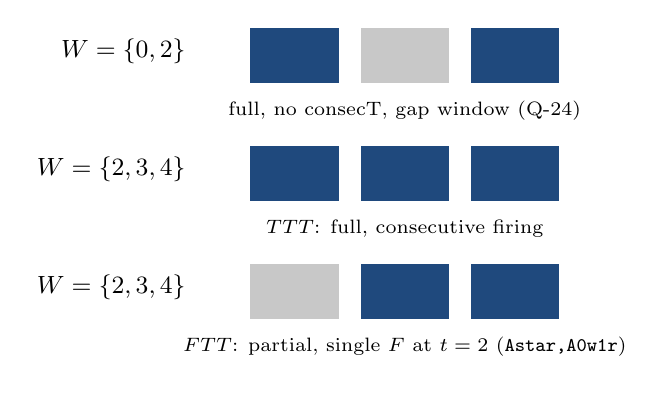
\begin{tikzpicture}[xscale=1.4, yscale=1]
    \definecolor{fire}{RGB}{31,73,125}
    \definecolor{idle}{RGB}{200,200,200}
    % W = {0,2}: full, no consecT
    \node[font=\small,anchor=east] at (-0.5,2.6) {$W=\{0,2\}$};
    \foreach \x/\c in {0/fire,1/idle,2/fire}
      \fill[\c] (\x,2.2) rectangle (\x+0.8,2.9);
    \node[font=\scriptsize] at (1.4,1.85) {full, no consecT, gap window (Q-24)};
    % W = {2,3,4}: TTT full
    \node[font=\small,anchor=east] at (-0.5,1.1) {$W=\{2,3,4\}$};
    \foreach \x in {2,3,4}
      \fill[fire] (\x-2,0.7) rectangle (\x-2+0.8,1.4);
    \node[font=\scriptsize] at (1.4,0.35) {$TTT$: full, consecutive firing};
    % W = {2,3,4}: FTT partial (A0w1r)
    \node[font=\small,anchor=east] at (-0.5,-0.4) {$W=\{2,3,4\}$};
    \fill[idle] (0,-0.8) rectangle (0.8,-0.1);
    \fill[fire] (1,-0.8) rectangle (1.8,-0.1);
    \fill[fire] (2,-0.8) rectangle (2.8,-0.1);
    \node[font=\scriptsize] at (1.4,-1.15) {$FTT$: partial, single $F$ at
      $t=2$ (\texttt{Astar,A0w1r})};
  \end{tikzpicture}
  \caption{Firing patterns on concrete frames (supplied datum, R280
    census): the Q-24 witness $W=\{0,2\}$ (top) is full yet has no
    consecutive firing times; $W=\{2,3,4\}$ with $\tau\equiv\lambda\equiv
    T$ realizes full/$TTT$ (\texttt{Astar,E3}) and partial/$FTT$
    (\texttt{Astar,A0w1r}, \texttt{Astar,N5w1}). Blue cells fire; gray
    cells do not.}
  \label{fig:frames}
\end{figure}

The repaired theory was audited computationally (R287, [COMPUTED]$\times2$,
zero shared code): the $472$-frame universe --- all complete frames with
$W\subseteq\{0,\dots,5\}$, $1\le|W|\le4$, every $\varepsilon$-pattern ---
contains $134$ consecutive-firing frames, $20$ gap-full frames (full
with no consecutive $T$'s, including the reviewer's $W=\{0,2\}$), and
$36$ consecutive-window-full frames; path~1 ran $1{,}398$ checks ALL
PASS, path~2 ran $1{,}262$ checks ALL PASS (supplied datum). The R280
concrete instances (supplied datum) are: $(\mathtt{Astar,E3})\to
(T,F,C)=(0,0,0)$, full, pattern $TTT$; $(\mathtt{Astar,A0w1r})$,
$(\mathtt{Astar,N5w1})\to(1,0,1)$, partial, pattern $FTT$ with the
single $F$ at $t=2$ ($\mathrm{edge}_{-9}=\{184\}$,
$\mathrm{edge}_{-1}=\{184\}$). The void pattern $FFF$ is absent from the
census --- an abstract prediction of the theory, not an input.

\begin{table}[t]
  \centering
  \caption{The $472$-frame R287 census (supplied [COMPUTED]$\times2$
    datum).}
  \label{tab:lockcensus}
  \begin{tabular}{lr}
    \toprule
    class & count \\
    \midrule
    total complete frames ($W\subseteq\{0,\dots,5\}$,
      $1\le|W|\le4$, all $\varepsilon$) & $472$ \\
    consecutive-firing frames & $134$ \\
    gap-full frames (full, $\varepsilon$ with no consecT) & $20$ \\
    consecutive-window-full frames & $36$ \\
    verification path~1 checks & $1{,}398$ (all pass) \\
    verification path~2 checks & $1{,}262$ (all pass) \\
    \bottomrule
  \end{tabular}
\end{table}

\begin{theorem}[D7$'$ dual-ascent barrier; PROVED, axiom-free]
  \label{thm:d7p}
  Let IsDual, IsDemoteEdge, IsPromoteEdge be as
  in~\eqref{eq:isdual}. Then:
  \begin{enumerate}
  \item[(a)] (\texttt{no\_dual\_target\_demote}) No demote edge targets
    a reflection dual of its source:
    \begin{equation}
      \label{eq:d7pa}
      \mathtt{IsDemoteEdge}(c,q)\ \land\ \mathtt{IsDual}(q,c)
      \ \Longrightarrow\ \bot.
    \end{equation}
  \item[(b)] (\texttt{no\_dual\_source\_promote}) No promote edge is
    sourced at a reflection dual of its target:
    \begin{equation}
      \label{eq:d7pb}
      \mathtt{IsPromoteEdge}(q,a)\ \land\ \mathtt{IsDual}(q,a)
      \ \Longrightarrow\ \bot.
    \end{equation}
  \end{enumerate}
\end{theorem}

The proof is pure finite order theory (T7$'$+A2): for (a), suppose
$q=(e',s)$ is a $\sigma$-dual of $c=(e,s)$; A2 gives the same $s$,
T7$'$ ($c\in\Pi(\sigma)$) gives $e'\ge e$; the demote orientation (D1,
$24/24$ scripted) gives $q\le c$, $q\neq c$, hence $e'\le e$; so
$e'=e$, $q=c$, contradicting $q\neq c$. Part (b) is symmetric. Both
theorems are \emph{axiom-free} ($0$ axioms, R294). The R288 census audit
([COMPUTED]$\times2$, zero shared code) found $0$ violations of
D7$'$(a) and $0$ of D7$'$(b) --- $0$ dual-related edges anywhere over
$294$ Pareto instances / $24$ demote $+$ $16$ promote edges (supplied
datum).

\begin{proposition}[Original D7 demoted to [OPEN]]
  \label{prop:q26}
  The original D7 (``no DAG edge relates a class to its reflection dual
  as distinct Pareto nodes'', a T8$'$ corollary conditional on T2$'$)
  does not follow from fixed-span T7$'$/T8$'$. Q-26's abstract
  non-entailment model (reconstructed in \texttt{r288\_reviewer\_model.py},
  all asserts pass; supplied datum): $S_\sigma=\{(5,5),(6,5)\}$ with
  swapped duals, $S_{\sigma+1}=\{(6,5)\}$ self-dual. Verified: T7$'$
  holds at both spans (Pareto duals have $e'\ge e$); T8$'$ holds at both
  spans (no distinct co-Pareto duals); T5 yields the promote edge
  $(5,5)\to(6,5)$ with blocker $(5,5)$; $(6,5)$ IS the $\sigma$-dual of
  $(5,5)$ --- so a DAG edge relates a class to its reflection dual as
  distinct Pareto nodes, and D7's conclusion FAILS. The broken step:
  ``hence never Pareto'' drops T8$'$'s same-$\sigma$ qualifier ---
  Pareto status is span-relative; fixed-span premises cannot constrain
  cross-span Pareto status. A second model realizes the demote-side
  half: $S_\sigma=\{(6,5),(7,5)\}$,
  $S_{\sigma+1}=\{(5,5),(6,5)\}$, demote edge $(6,5)\to(5,5)$ with
  $(6,5)$ a $(\sigma{+}1)$-dual of $(5,5)$.
\end{proposition}

\begin{figure}[t]
  \centering
  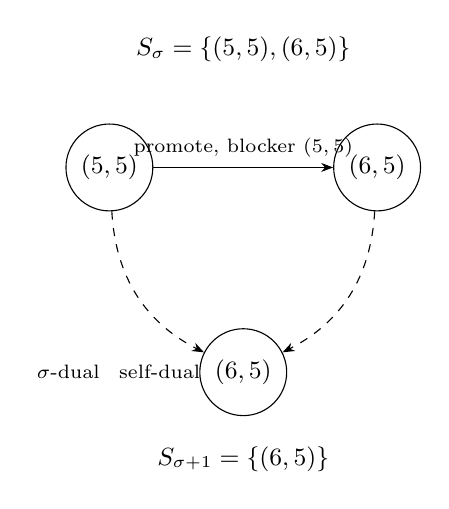
\begin{tikzpicture}[
      node distance=1.8cm,
      cls/.style={draw, circle, minimum size=1.1cm, font=\small},
    ]
    \node[cls] (a) at (0,2.6) {$(5,5)$};
    \node[cls] (b) at (3.4,2.6) {$(6,5)$};
    \node[cls] (c) at (1.7,0) {$(6,5)$};
    \draw[-{Stealth[scale=0.9]}] (a) -- (b)
      node[midway,above,font=\scriptsize] {promote, blocker $(5,5)$};
    \draw[-{Stealth[scale=0.9]},dashed] (a) to[bend right=30] (c)
      node[midway,left,font=\scriptsize] {$\sigma$-dual};
    \draw[-{Stealth[scale=0.9]},dashed] (b) to[bend left=30] (c)
      node[midway,right,font=\scriptsize] {self-dual};
    \node[font=\small] at (1.7,4.1) {$S_\sigma=\{(5,5),(6,5)\}$};
    \node[font=\small] at (1.7,-1.1) {$S_{\sigma+1}=\{(6,5)\}$};
  \end{tikzpicture}
  \caption{Q-26's abstract non-entailment model (Proposition~\ref{prop:q26}):
    T7$'$ and T8$'$ hold at both spans, yet the promote edge
    $(5,5)\to(6,5)$ relates a class to its reflection dual as a distinct
    Pareto node. Fixed-span premises cannot constrain cross-span Pareto
    status, so the original D7 is [OPEN], not a theorem (supplied datum,
    R288 dossier).}
  \label{fig:q26model}
\end{figure}

The conditional D7$''$ --- dual non-domination
$H$: ``no Pareto $q\in\Pi(\sigma)$ has a DISTINCT dual
$d\in S(\sigma)$ with $q\le d$'' implies the full D7 --- is recorded as
[PROVED* conditional] but \emph{inapplicable}: $H$ is FALSE on the
census ($39$ violations, e.g.\ $\sigma=81$: $(37,1)$ Pareto dominates its
dual $(47,1)\in S(81)$; $H_{\mathrm{sym}}$ fails with $3$ violations;
$15$ self-dual Pareto instances; supplied datum). The complementary
halves (promote target $=$ dual of source; demote source $=$ dual of
target) stay [OPEN] --- abstract models realize both, so the full D7 is
contingent, not a theorem.

\begin{theorem}[$L_s$/C3 ascent-depth bounds; PROVED]
  \label{thm:ascent}
  Over a finite vertex type $V$ with promote relation $E_p$ and
  $\mathtt{PromoAcyclic}$ (R292's D1b):
  \begin{enumerate}
  \item[($L_s$)] (\texttt{dual\_preserves\_s\_card}) Reflecting a finset
    in a bound preserves card: for all $\sigma$ and
    $W\subseteq\mathbb{N}$ finite with $w\le\sigma$ on $W$,
    \begin{equation}
      \label{eq:ls}
      \bigl(W.\mathrm{image}(w\mapsto\sigma-w)\bigr).\mathrm{card}
      =W.\mathrm{card},
    \end{equation}
    the order-theoretic core of ``duals preserve $s$''
    ($W(\bar A)=\sigma-W(A)$, $w\mapsto\sigma-w$ bijecting
    $[0,\sigma]$).
  \item[(C3-i)] (\texttt{ascentDepth\_le})
    $\mathtt{ascentDepth}(c)\le|V|-1$ for all $c$.
  \item[(C3-ii)] (\texttt{ascentDepth\_promote\_mono})
    $E_p(q,a)$ implies
    $\mathtt{ascentDepth}(a)+1\le\mathtt{ascentDepth}(q)$: ascent depth
    strictly increases against the promote direction (prepend $q$ to a
    longest chain from $a$; $q$ is fresh, else a positive closed walk
    against acyclicity).
  \item[(C3-iii)] (\texttt{ascentDepth\_eq\_zero\_iff})
    $\mathtt{ascentDepth}(c)=0\iff\forall a,\ \lnot E_p(c,a)$: zero
    depth iff $c$ sources no promote edge.
  \end{enumerate}
\end{theorem}

Theorem~\ref{thm:ascent} is R292's $L_s$/C3 suite folded into
\texttt{TransDAG.lean} in R298, [PROVED] in R310 with standard axioms.
Q-36 (Bunny, quoted verbatim 2026-10-11~03:14--03:35~PDT): ``$L_s$
SURVIVES'' and ``C3 SURVIVES (finite promotion DAGs, bound
$|C|-1)$'', scoped to finite promotion DAGs; C1/C2/C4 received
OBJECTION and are not claimed.

%======================================================================
\section{Discussion}
%======================================================================

\paragraph{Significance.} The abstract-lock theory shows how little is
needed to force firing structure: from a window and three predicates,
the repaired laws (Theorem~\ref{thm:locks}) recover the exact
boundary between consecutive-firing, scattered-firing, and gap-window
regimes, and the Q-24 witness proves the boundary is sharp. The $472$-
frame census (Table~\ref{tab:lockcensus}) is a genuine discovery of the
abstract theory: $20$ gap-full frames exist, and the void $FFF$ pattern
never occurs. The dual-ascent barrier (Theorem~\ref{thm:d7p}) is the
strongest statement that survives the Q-26 objection --- axiom-free
pure order theory, audited at $0$ violations over $294$ Pareto
instances. The $L_s$/C3 suite turns the transition DAG's promote edges
into a well-founded ascent-depth measure bounded by $|C|-1$.

\paragraph{The refutation record.} We keep both objections visible
because the repairs are the paper's real content. The original T3(iii)
fell to a two-point window ($W=\{0,2\}$); the surviving content is the
sharp window-conditional form (c)(i)/(c)(ii), and the Lean
\texttt{sharpness\_witness} is the counterexample promoted into a
theorem about premise necessity. The original D7 fell to an abstract
model with swapped duals; the surviving content is the axiom-free
barrier D7$'$ (the two halves that follow from T7$'$+A2 alone), while
the conditional D7$''$ is recorded but inapplicable ($H$ false on the
census) and the complementary halves stay [OPEN]. This is the honest
boundary: D7$'$ is not a recovery of D7.

\paragraph{Limitations.} (i) The dual-ascent barrier's premises
(T7$'$ with $s$-preservation at both spans) are abstract hypotheses;
the $195$-class Sidon census application is explicitly out of scope
per Q-33. (ii) The abstract-lock census covers only $W\subseteq
\{0,\dots,5\}$ with $|W|\le4$ --- the sharpness claims generalize by
proof, but the empirical pattern (void $FFF$ absent) is a census
observation, not a theorem. (iii) Q-32's scope is ``complete finite
nonempty frames with integer adjacency''; partial frames are not
covered. (iv) The transition-DAG definitions (merges, splits, the
$(14,4)\rightleftarrows(14,5)$ flip-flop) and the $24/16/14$
edge counts are supplied [COMPUTED] datums, not formalized.

%======================================================================
\section{Conclusion}
%======================================================================

We have proved in Lean the repaired consecutive-firing laws for
abstract locks (Theorem~\ref{thm:locks}, [PROVED]), the axiom-free
dual-ascent barrier for transition DAGs (Theorem~\ref{thm:d7p},
[PROVED]), and the $L_s$/C3 ascent-depth bounds
(Theorem~\ref{thm:ascent}, [PROVED]), all with zero sorrys on the
bakkie full-library build. The refutations that shaped the repairs ---
Q-24's $W=\{0,2\}$ counterexample and Q-26's abstract non-entailment
model --- are reported honestly and, where possible, promoted into
sharpness theorems. What remains open: the complementary halves of the
full D7 barrier, the inapplicable conditional D7$''$, the C1/C2/C4
fragments (all OBJECTION), and the census application of D7$'$ (Q-33
OBJECTION stands until full-spectrum endpoints or a proved all-duals
ascent is available).

%======================================================================
\section{References}
%======================================================================

\begin{thebibliography}{9}

\bibitem{ERS66}
P.~Erd\H{o}s, A.~R\'enyi, and V.~T.~S\'os,
\emph{On a problem of graph theory},
Studia Sci.\ Math.\ Hungar.\ \textbf{1} (1966), 215--235.
(The friendship theorem, cited as given among the program's classical
references, R298.)

\bibitem{ET41}
P.~Erd\H{o}s and P.~Tur\'an,
\emph{On a problem of Sidon in additive number theory},
J. London Math.\ Soc.\ \textbf{16} (1941), 212--215.
(Cited as given among the program's classical Sidon references.)

\bibitem{OpenAI}
OpenAI,
\emph{github.com/openai/math} catalogue,
$719$ manuscripts fetched 2026-10-10, $0$ ``Sidon'' hits
(cited as given, R273/R279 novelty checks; the $\sigma$-spectrum and
its transition DAG are program-defined objects).

\bibitem{D280}
D.~Blair,
\emph{Unsolved Math --- Round 280: abstract lock theory},
program dossier, 2026-10-10.
(Supplied datum: lock-frame definitions, Q-24 OBJECTION, concrete
instances, $472$-frame census design.)

\bibitem{D287}
D.~Blair,
\emph{Unsolved Math --- Round 287: repaired lock laws},
program dossier, 2026-10-11.
(Supplied datum: T3(iii$'$) repair, quantifier-slip mechanism, Q-32
verdict, [COMPUTED]$\times2$ census.)

\bibitem{D279}
D.~Blair,
\emph{Unsolved Math --- Round 279: transition DAG census},
program dossier, 2026-10-10.
(Supplied datum: $G=(C,E_d\cup E_p\cup\mathcal{L})$ census, $24/16/14$
edge counts, merges/splits, flip-flop.)

\bibitem{D288}
D.~Blair,
\emph{Unsolved Math --- Round 288: D7$'$ dual-ascent barrier},
program dossier, 2026-10-11.
(Supplied datum: Q-26 model, broken-step location, D7$'$ proofs,
D7$'$/$H$/$H_{\mathrm{sym}}$ audits, Q-33 verdict.)

\bibitem{D298}
D.~Blair,
\emph{Unsolved Math --- Round 298: queue hardening},
program dossier, 2026-10-10.
(Supplied datum: md5 sync records, $L_s$/C3 fold, Q-36 verdict.)

\bibitem{D310}
D.~Blair,
\emph{Unsolved Math --- Round 310: full-library build gate},
program dossier, 2026-10-11.
(Supplied datum: bakkie \texttt{lake build} ``Build completed
successfully (17936 jobs)'', exit~0, $0$ errors, $0$ sorrys;
label moves.)

\end{thebibliography}

\end{document}

% --- WEAKNESSES (substantive) ---
% 1. The dual-ascent barrier's premises (T7'+s-preservation at both spans)
%    are abstract hypotheses; the census application that motivated D7'
%    is explicitly out of scope (Q-33), so the theorem is a conditional
%    whose condition the paper never discharges.
% 2. The abstract-lock census covers only W in {0..5} with |W|<=4 — the
%    sharpness claims generalize by proof, but the empirical pattern
%    (void FFF absent) is a census observation, not a theorem.
% 3. D7' leaves the two complementary halves [OPEN] and D7'' inapplicable
%    (H false on census); the repaired barrier is weaker than the
%    original D7 ambition and must not be read as recovering it.
%
% --- TYPOGRAPHY ISSUES NOTICED ---
% 1. Long Lean theorem names in prose (e.g. \texttt{full_no_consecT_gap_
%    window}) break lines badly; an abbreviation table or shorter
%    display aliases would typeset more cleanly.
% 2. Verdict labels mix styles (Q-24, Q-32, Q-33 as bare text); a uniform
%    macro (e.g. \textsc or \texttt) would keep them consistent.
% 3. The symbol W denotes both the firing window and appears in the
%    W(bar A) mechanism discussion; the two uses should be disambiguated
%    typographically.
